\begin{figure}[tp]
	\centering
	\begin{lrbox}{\mintedbox}
		\begin{minipage}{0.48\textwidth}
			\tscode{code/background/typescript/declaration-files/calculator-error-index.d.ts}
		\end{minipage}
	\end{lrbox}
	\subfloat[calculator/index.d.ts]{\usebox{\mintedbox}}
	\hfill
	\begin{lrbox}{\mintedbox}
		\begin{minipage}{0.48\textwidth}
			\jscode{code/background/typescript/declaration-files/calculator-index.js}
		\end{minipage}
	\end{lrbox}
	\subfloat[calculator/index.js]{\usebox{\mintedbox}}

	\subfloat[Visual Studio Code auto-completion]{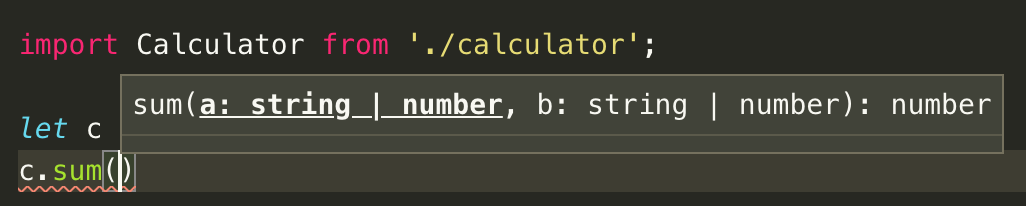
\includegraphics[width=0.8\textwidth]{figures/background/typescript/declaration-files/ide-auto-completion-error.png}}

	\begin{lrbox}{\mintedbox}
		\begin{minipage}{0.58\textwidth}
			\jscode{code/background/typescript/declaration-files/calculator-error-index.ts}
		\end{minipage}
	\end{lrbox}
	\subfloat[index.ts]{\usebox{\mintedbox}}
	\hfill
	\begin{lrbox}{\mintedbox}
		\begin{minipage}{0.4\textwidth}
			\begin{bashinline}
$ tsc index.ts
$ node index.js
Error: Only numbers are allowed!
			\end{bashinline}
		\end{minipage}
	\end{lrbox}
	\subfloat[Console output]{\usebox{\mintedbox}}

	\caption[TypeScript declaration file with errors]{\textbf{TypeScript declaration file with errors} - An error is explicitly introduced by writing in the declaration file that the \mintinline{text}{sum} method accepts also a \mintinline{text}{string}. IDE and compiler blindly trust the declaration file. An error occurs only at run-time.}
	\label{fig:background-declaration-files-calculator-error-example}
\end{figure}